% This file was created by matlab2tikz.
%
%The latest updates can be retrieved from
%  http://www.mathworks.com/matlabcentral/fileexchange/22022-matlab2tikz-matlab2tikz
%where you can also make suggestions and rate matlab2tikz.
%
\documentclass[tikz]{standalone}
\usepackage[T1]{fontenc}
\usepackage[utf8]{inputenc}
\usepackage{pgfplots}
\usepackage{grffile}
\pgfplotsset{compat=newest}
\usetikzlibrary{plotmarks}
\usepgfplotslibrary{patchplots}
\usepackage{amsmath}
\usetikzlibrary{decorations.markings}
\definecolor{mycolor1}{rgb}{0.00000,0.44700,0.74100}%
\definecolor{mycolor2}{rgb}{0.85000,0.32500,0.09800}%
\begin{document}

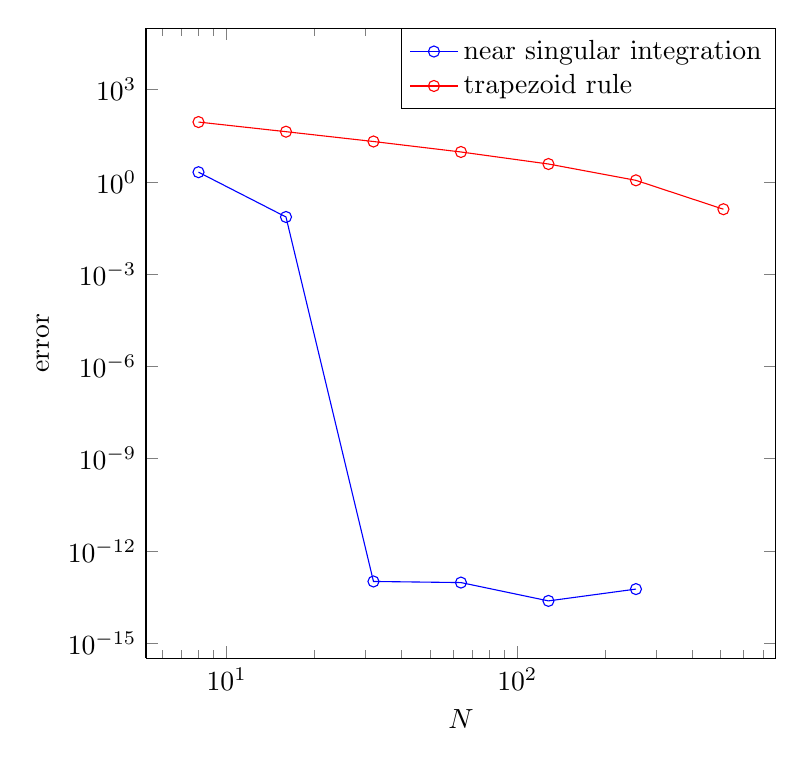
\begin{tikzpicture}

\begin{axis}[%
width=8cm,
height=8cm,
scale only axis,
separate axis lines,
every outer x axis line/.append style={black},
every x tick label/.append style={font=\color{black}},
xmode=log,
xminorticks=true,
xlabel={$N$},
ymode=log,
ymax=10e4,
yminorticks=true,
ylabel={error},
axis background/.style={fill=white},
legend style={legend cell align=left,align=left,draw=black, at={(1,1)}, anchor=north east}
]
\addplot [color=blue,solid,mark=o,mark options={solid}]
  table[row sep=crcr]{%
  8     2.08e0\\
  16  7.27e-2\\
  32  1.02e-13\\
  64  9.38e-14\\
  128 2.38e-14\\
  256 5.76e-14\\
};
\addlegendentry{near singular integration};

\addplot [color=red,solid,mark=o,mark options={solid}]
  table[row sep=crcr]{%
  8     8.89e1\\
  16   4.32e1\\
  32  2.07e1\\
  64 9.45e0\\
  128 3.84e0\\
  256 1.13e0\\
 512 1.30e-1\\
};
\addlegendentry{trapezoid rule};


\end{axis}
\end{tikzpicture}%
\end{document}